\chapter{Adaptación al problema de Selección de Instancias}
\label{capitulo3}
\lhead{Capítulo 3. \emph{Adaptación al problema de Selección de Instancias}}

Al tratarse de métodos de búsqueda de propósito general, las metaheurísticas pueden modificarse para encontrar soluciones a todo tipo de problemas de optimización combinatoria. Para ello debe definirse la representación a usar, que permita codificar las posibles soluciones al problema, y una función de \emph{fitness} para evaluar dichas soluciones en función a los objetivos de optimización del problema.

A continuación se describen éstas y otras consideraciones generales para la aplicación de metaheurísticas al problema de \emph{Selección de Instancias}. Adicionalmente se plantea para cada metaheurística, las estrategias a usar durante el proceso de búsqueda, así como algunas modificaciones particulares.

\section{Consideraciones generales}

\subsection{Representación}

Una solución cualquiera al problema de \emph{SI} está dada por un subconjunto de instancias $R$ del conjunto inicial $T$ (\emph{i.e.} $R \subseteq T$). Por lo tanto, para un orden dado de las instancias $t_i \in T\ (i = 1 \dots n$, con $n = \vert T \vert)$, una codificación usando mapas de bits es suficiente para representar el espacio de soluciones al problema.

En este sentido, una solución particular al problema de \emph{SI} está descrita por un cromosoma $s$ de tamaño $n$, donde cada gen $s_i$ ($i = 1 \dots n$) es un \emph{bit} con valor 1/0 (``prendido'' o ``apagado'' respectivamente) que denota la pertenencia o no de la instancia correspondiente $t_i \in T$ al subconjunto seleccionado. $R_s \subseteq T$ es el subconjunto seleccionado representado por el cromosoma $s$, donde:

\begin{equation}
R_s = \left\lbrace t_i \in T \mid i = 1 \dots n \land s_i = 1 \right\rbrace
\end{equation}

Este conjunto $R_s$ permite evaluar la ``bondad'' de la solución $s$ en función de los objetivos de optimización del problema.

\subsection{Función de evaluación}

El objeto de la aplicación de metaheurísticas es conseguir soluciones óptimas o casi óptimas a gran variedad de problemas. Para ello es necesario definir una estrategia de comparación entre soluciones, \emph{i.e.} saber cuándo una solución es \guillemotleft\emph{mejor}\guillemotright\ que otra, que permita seleccionar aquellas soluciones que mejor se adapten a los objetivos del problema en cuestión.

Para el caso del problema de \emph{SI}, el objetivo es encontrar un subconjunto $R$ del menor tamaño posible, que mantenga un alto porcentaje de precisión de clasificación. \emph{Cano et al.} \cite{cano2003using} definen una función de evaluación que combina ambos objetivos en función de un parámetro $\alpha \in [0,1]$; a continuación se presenta una modificación de dicha función (su complemento), usada en el presente trabajo:

\begin{equation}
\mathit{fitness}(R) = \alpha\ \mathit{error}(R) + (1 - \alpha) \vert R \vert
\end{equation}

Donde $\mathit{error}(R)$ es el número de instancias en $T$ que son erróneamente clasificadas usando el conjunto $R \subseteq T$ como conjunto de entrenamiento de un clasificador 1-NN. El parámetro $\alpha$ combina los objetivos de la búsqueda: se usa $\alpha = 0.5$ siguiendo lo descrito por \cite{cano2003using} para obtener soluciones que satisfagan ambos objetivos del problema.

Para esta definición, el objetivo de las metaheurísticas para selección de instancias es \emph{minimizar} la función de evaluación descrita. Para ello deben minimizar ambos objetivos de la función; el error de clasificación usando el subconjunto seleccionado, y el tamaño de dicho subconjunto. En este sentido, dadas dos posibles soluciones $a$ y $b$, $a$ es \guillemotleft\emph{mejor}\guillemotright\ que $b$ si y solo si $\mathit{fitness}(R_a) < \mathit{fitness}(R_b)$.

\subsection{Generación de soluciones iniciales}
\label{generacion-sol-inic}

Para muchos problemas con esquemas de representación binaria, la generación de soluciones iniciales usada por metaheurísticas sigue una estrategia común: al generar un cromosoma aleatorio, cada bit tiene $50\%$ de probabilidad de estar prendido ($\delta = 0.5$). Esta estrategia genera soluciones con valor esperado de la mitad de los bits prendidos. Para el problema de \emph{SI} esto implica soluciones con una reducción inicial del $50\%$ sobre el conjunto $T$, y hace necesario un alto número de iteraciones para lograr obtener soluciones con reducciones significativas \cite{cano2003using}. Por esta razón, en el presente trabajo se usa una probabilidad de aparición del $5\%$ por cada bit ($\delta = 0.05$), generando soluciones iniciales con reducciones cercanas al $95\%$; el rol de la función objetivo no recae en disminuir los porcentajes de reducción de las soluciones, sino en mantenerlos en niveles aceptables, permitiendo explotar el espacio de búsqueda para conseguir soluciones con mayor precisión.

Sin embargo, el punto inicial de la búsqueda en términos de precisión sigue siendo aleatorio. Una estrategia común en metaheurísticas de trayectoria es la generación de soluciones iniciales usando algoritmos de aproximación; \emph{Cerveron et al.} \cite{cerveron2001another} plantean una modificación del algoritmo de Búsqueda Tabú para el problema de \emph{SI}, en la cuál usan CNN para generar la solución inicial de la búsqueda. Esta idea puede trasladarse a metaheurísticas poblacionales siguiendo un enfoque probabilístico: dada una selección inicial $R_0 \subseteq T$, los bits correspondientes a instancias en $R_0$ tienen mayor probabilidad de aparición que los bits de instancias en $T \setminus R_0$. Estas probabilidades constituyen un vector de probabilidades a ser usado por PBIL como vector inicial, o por los algoritmos genéticos (GGA, SGA y CHC) para generar soluciones iniciales. El algoritmo \ref{inicial-sol-alg} implementa este esquema de generación; para un $\delta$ particular (que determina el número de bits prendidos en las soluciones iniciales), el vector de probabilidades $V$ generado por el algoritmo cumple con que un máximo del $70\%$ de los bits prendidos en soluciones generadas usando $V$, pertenecen a la solución inicial $R_0$. Esto contribuye a guiar la búsqueda realizada por las metaheurísticas poblacionales, mientras se mantiene la variabilidad.

\begin{algorithm}
\caption{Generador de vector de probabilidades inicial}
\label{inicial-sol-alg}
\begin{algorithmic}[1]

\Require $R_0$ solución inicial
\Ensure Vector de probabilidades en base a $R_0$

\State{$high \gets min(0.9, \frac{\delta \vert T \vert 0.7}{\vert R_0 \vert})$}
\State{$low \gets \frac{\delta \vert T \vert - hi \vert R_0 \vert}{\vert T \setminus R_0 \vert}$}
\State{$V \gets$ Vector de probabilidades de tamaño n}
\For{$i \in [1 \dots n]$}
	\If{$t_i \in R_0$}
		\State{$V_i \gets high$}
	\Else
		\State{$V_i \gets low$}
	\EndIf
\EndFor
\State \Return{$V$}
\end{algorithmic}
\end{algorithm}

Cualquier solución generada por algoritmos de aproximación para el problema de \emph{SI} (sección \ref{alg-aprox-si}) sirve como ``semilla'' de este generador; en el presente trabajo se prueba el impacto del uso de soluciones iniciales calculadas por CNN. También se incluyen dos selecciones basadas en el orden según el \emph{enemigo más cercano} (NE - ``\emph{Nearest Enemy}''), seleccionando las instancias con mayor distancia NE (selección por \emph{Farthest NE}), o menor distancia NE (selección por \emph{Closest NE}). Finalmente, se prueba un método de selección propio llamado \emph{Nearest Enemy Hypersphere Selection} (NEHS). En la figura \ref{seleccion} se pueden observar los subconjuntos seleccionados por estas cuatro (4) estrategias.

\begin{figure}[h!]
\centering
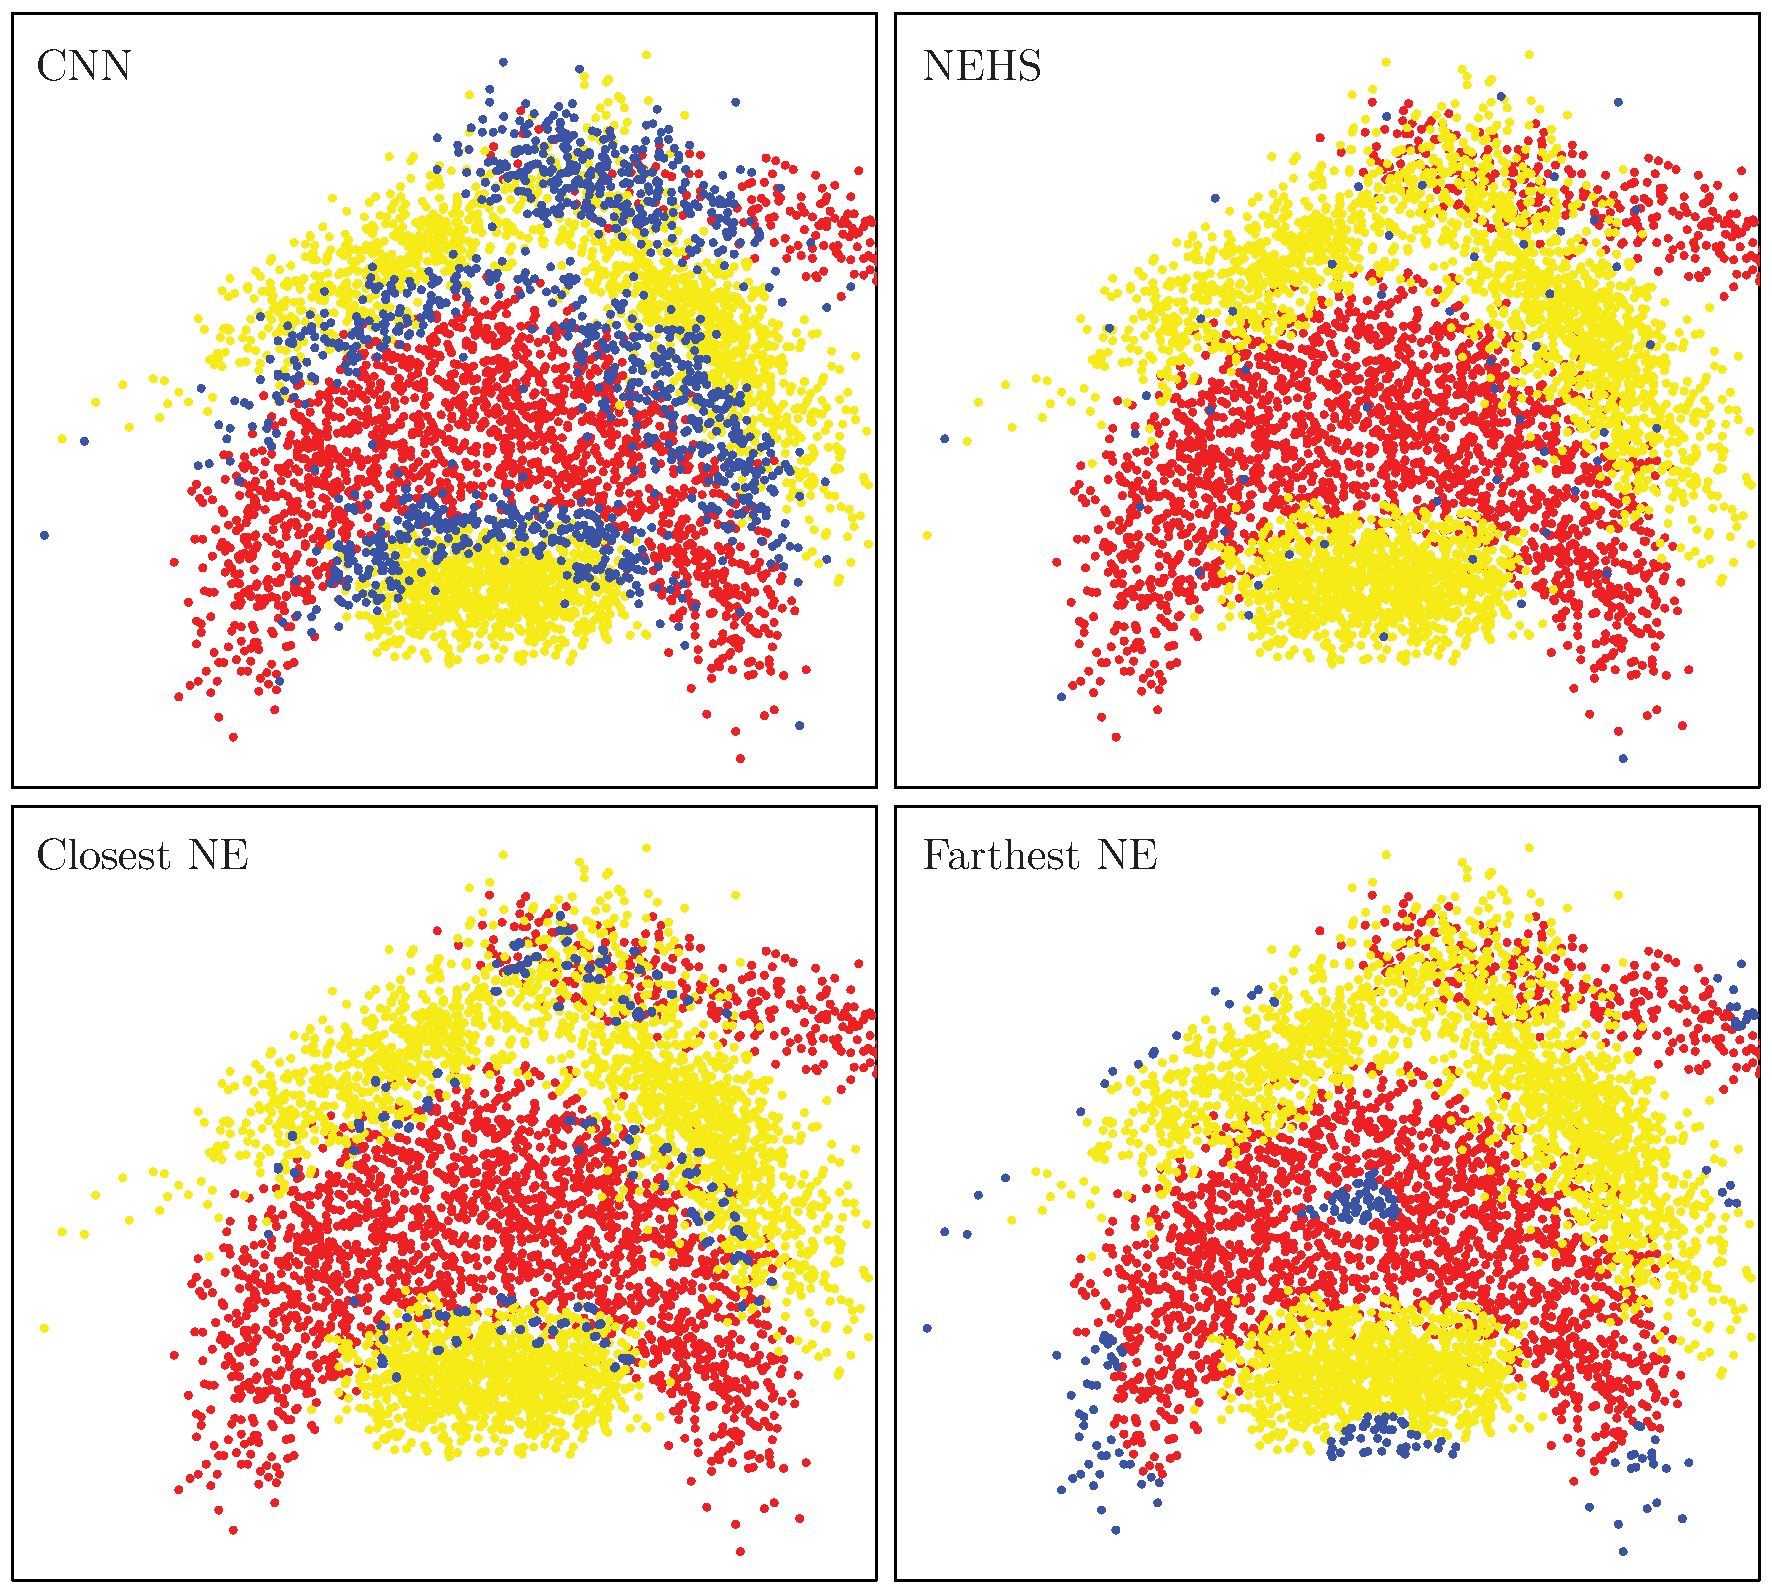
\includegraphics[width=0.8\textwidth]{seleccion.pdf}
\caption[Algoritmos de Selección de Instancias]{Subconjunto de instancias seleccionadas por CNN, NEHS, Closest NE y Farthest NE, para el conjunto de instancias \textsc{Banana}. Las instancias están pintadas en amarillo y rojo según su clase en el conjunto de datos, y en azul aquellas instancias pertenecientes a la selección correspondiente.}
\label{seleccion}
\end{figure}

\subsubsection{Condensed Nearest Neighbor}

En 1968 \emph{Hart} \cite{Hart:2006:CNN:2263267.2267647} fue el primero en proponer un método de reducción de instancias a ser usadas por la regla NN; este método se conoce como \emph{Condensed Nearest Neighbor} (CNN). El objetivo de CNN es realizar un proceso de selección previo al entrenamiento del clasificador 1-NN, consiguiendo un conjunto $R \subseteq T$ que mantenga la efectividad del conjunto de datos original $T$ para clasificar instancias desconocidas.

Se trata de un algoritmo incremental en el que se incluyen en $R$ aquellas instancias en $T$ que son mal clasificadas usando conjunto reducido como conjunto de entrenamiento en un clasificador 1-NN. Dicho proceso se repite hasta que no se incluyan nuevas instancias en el conjunto $R$ luego de una iteración completa sobre las instancias en $T$; ver algoritmo \ref{cnn-alg}.

\begin{algorithm}
\caption{Condensed Nearest Neighbor}
\label{cnn-alg}
\begin{algorithmic}[1]

\Require $T$ conjunto de instancias inicial
\Ensure Conjunto de instancias $R \subseteq T$

\State $R \gets \left\lbrace \mathrm{Una\ instancia\ cualquiera}\ t \in T \right\rbrace$
\Repeat
	\State $R' \gets R$
	\ForAll{$t \in T$}
		\If{$t$ es mal clasificada usando $R$ con un clasificador 1-NN}
			\State $R \gets R \cup \left\lbrace t \right\rbrace$
		\EndIf
	\EndFor
\Until{$R = R'$}
\State \Return{$R$}
\end{algorithmic}
\end{algorithm}

CNN logra una reducción considerable sobre el conjunto de datos original, y asegura un conjunto consistente con $T$. Sin embargo, al ser dependiente del orden de revisión de las instancias, CNN no asegura un conjunto consistente \emph{mínimo}. Este algoritmo tiende a seleccionar instancias cercanas a los bordes de decisión, viéndose particularmente afectado por datos ruidosos \cite{amal2011survey, Jankowski_comparisonof}.

\subsubsection{Nearest Enemy Hypersphere Selection}

La idea tras el uso de la regla NN es que instancias ``cercanas'' en un espacio cualquiera (\emph{i.e.} con atributos similares) comparten su clasificación; esto conlleva a la división de dicho espacio en regiones con instancias de igual clase. La idea fundamental de \emph{Nearest Enemy Hypersphere Selection} (NEHS) es seleccionar instancias en los centros de dichas regiones, con la finalidad de reducir la cantidad de instancias necesarias para generalizar el espacio descrito por el conjunto original.

Para esto hace uso de la distancia del \emph{enemigo más cercano}: cada instancia $t \in T$ tiene un enemigo más cercano $\mathrm{NE}(t) \in T$, cuya distancia $\varphi(t,\mathrm{NE}(t))$ define el radio de una hiperesfera en el espacio $m$-dimensional de atributos con centro en $t$, dentro de la cual toda instancia comparte la clase $\omega_t$.

\begin{figure}[h!]
\centering
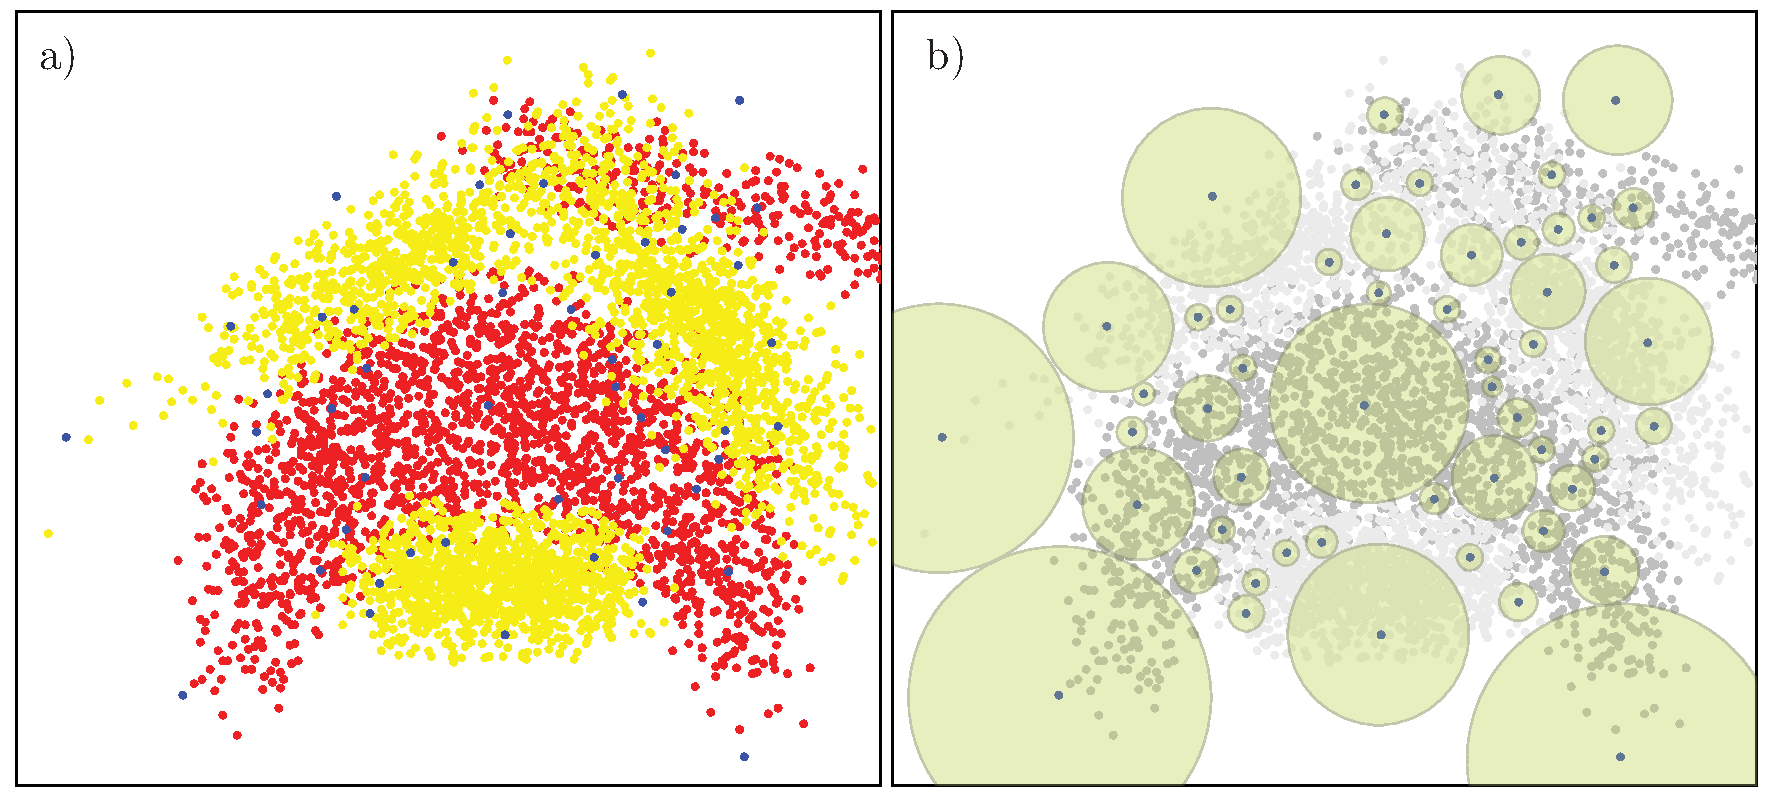
\includegraphics[width=0.8\textwidth]{hiperesferas.pdf}
\caption[Selección obtenida por NEHS]{a) Subconjunto de instancias seleccionadas por NEHS, e\\b) Hiperesferas correspondientes a la selección de NEHS, con radio en\\función a la distancia del enemigo más cercano.}
\label{seleccion}
\end{figure}

NEHS implementa una estrategia \emph{greedy} que busca seleccionar las mayores hiperesferas que no intersecten entre sí. Realiza la selección de hiperesferas comenzando con las de mayor tamaño, con el objetivo de cubrir el mayor espacio posible (ver el algoritmo \ref{necs-alg}). Sin embargo, para evitar la selección de puntos cercanos a los bordes de decisión (y posiblemente ruidosos), NEHS ignora un porcentaje $\Delta$ de instancias en $T$ con menor distancia NE, \emph{i.e.} las hiperesferas de menor radio. Esto implica una selección con bordes de decisión mucho más ``suaves'' que los del conjunto original.

\begin{algorithm}
\caption{Nearest Enemy Hypersphere Selection}
\label{necs-alg}
\begin{algorithmic}[1]

\Require $T$ conjunto de instancias inicial, $\Delta$ porcentaje de instancias a excluir
\Ensure Conjunto de instancias $R \subseteq T$

\State $R \gets \emptyset$
\ForAll{$t \in T$ en orden descendiente de distancia NE\par
	\hskip\algorithmicindent excluyendo las últimas $\Delta\vert T \vert$ instancias}
	\If{$\lnot\exists\ r \in R$ tal que $\varphi(t,r) < \varphi(r,\mathrm{NE}(r)) + \varphi(t,\mathrm{NE}(t))$}
		\State $R \gets R \cup \left\lbrace t \right\rbrace$
	\EndIf
\EndFor
\State \Return{$R$}
\end{algorithmic}
\end{algorithm}

\subsubsection{Closest Nearest Enemy}

La distancia del \emph{enemigo más cercano} (NE) de una instancia cualquiera $t \in T$ (\emph{i.e.} $\varphi(t,\mathrm{NE}(t))$), indica su cercanía a los bordes de decisión establecidos mediante un clasificador 1-NN. La selección por \emph{Closest NE} escoge aquellas instancias con \emph{menor} distancia NE entre las instancias en $T$, \emph{i.e.} instancias pertenecientes --o cercanas-- a los bordes de decisión de los datos. En el presente trabajo, \emph{Closest NE} selecciona el $5\%$ ($\delta = 0.05$) de instancias con menor distancia NE.

\begin{equation}
R_\mathrm{ClosestNE} = \left\lbrace \delta \vert T \vert\ \mathrm{instancias\ con\ menor\ distancia\ NE} \right\rbrace
\end{equation}

\subsubsection{Farthest Nearest Enemy}

Similar a la selección por \emph{Closest NE}, \emph{Farthest NE} se basa en el uso de la distancia NE para incluir instancias en el conjunto reducido $R \subseteq T$. Sin embargo, \emph{Farthest NE} selecciona aquellas instancias con \emph{mayor} distancia NE, \emph{i.e.} instancias alejadas de los bordes de decisión y cercanas a los centros de sus respectivas regiones. Este método también usa un porcentaje de selección igual al $5\%$ ($\delta = 0.05$) de las instancias en $T$.

\begin{equation}
R_\mathrm{FarthestNE} = \left\lbrace \delta \vert T \vert\ \mathrm{instancias\ con\ mayor\ distancia\ NE} \right\rbrace
\end{equation}

\section{Modificaciones particulares}

\subsection{Adaptación de GGA, SGA y CHC}

Para aplicar algún algoritmo genético al problema de \emph{SI}, es necesario describir las estrategias de selección, recombinación, mutación y reemplazo que seguirá el algoritmo durante el proceso evolutivo.

GGA, SGA y CHC requieren de un operador que seleccione individuos de la población para participar en el proceso reproductivo. Se emplea el método de \emph{selección por torneo} en su versión ``determinista'': se escoge al azar un conjunto de individuos entre la población original, y es seleccionado el más apto entre ellos. El tamaño de dicho conjunto debe ser pequeño; generalmente se usa un ``tamaño de torneo'' entre 2 y 5 \cite{Miller95geneticalgorithms}. En este trabajo se usan torneos de tamaño 3.

Debido a que CHC aplica un operador de recombinación particular (HUX) y no requiere de un operador de mutación, dichos operadores deben ser definidos solo para GGA y SGA. El operador de \emph{crossover} aplicado en ambos algoritmos es el \emph{recombinación en un punto}. Dados dos cromosomas ``padres'', se elige aleatoriamente un punto de corte en la longitud de ambos cromosomas; los cromosomas ``hijos'' resultan de combinar la sección izquierda del corte de un padre, con la sección derecha del corte del otro padre. El operador de mutación sigue --en ambos casos-- el esquema estándar de modificación de cada bit con una cierta probabilidad.

Finalmente, es necesario describir los criterios de reemplazo. Al tratarse de estrategias evolutivas generacionales, GGA y CHC reemplazan la población de forma incondicional en favor de la descendencia. En cambio, el criterio de reemplazo usado en SGA es ``elitista''; se sustituyen los padres por la descendencia generada, solo si dicha descendencia es mejor.

\subsection{Adaptación de PBIL}

La estrategia evolutiva de PBIL no requiere modificaciones adicionales para su aplicación al problema de selección de instancias; está diseñado para encontrar soluciones con representación binaria, lo que permite su aplicación directa al problema. La única modificación realizada al esquema estándar de PBIL es en el método de generación del vector de probabilidades iniciales, reflejando lo descrito en la sección \ref{generacion-sol-inic}.

\subsection{Adaptación de PSO}

La adaptación de PSO al problema de \emph{SI} es mayor, debido a que PSO está pensado para problemas con representación en espacios euclidianos; \emph{i.e.} es necesario el mapeo de vectores en $\mathbb{R}^l$ a soluciones con representación binaria. En este sentido, se adopta el esquema poblacional de PBIL en el que el genotipo de la población se representa de forma probabilística.

A esta adaptación de PSO la llamaremos \emph{Population-Based PSO} (ver algoritmo \ref{pbpso-alg}), en la cuál el vector de posición $\vec{X_i}$ de cada partícula es un vector de probabilidades que representa el genotipo de una población particular. Esto permite la generación de soluciones en codificación binaria para su respectiva evaluación, en base al vector de probabilidades que describe dicha población. A diferencia del PSO tradicional, la selección de óptimos locales y globales se hace en base a las soluciones generadas mediante $\vec{X_i}$, y no en base al vector $\vec{X_i}$ por si solo. Sin embargo, la modificación de los vectores de probabilidad y velocidad ($\vec{X_i}$ y $\vec{V_i}$ respectivamente) sigue la estrategia de actualización estándar en base a la mejor solución local y la mejor solución global.

\begin{algorithm}
\caption{Population-Based PSO}
\label{pbpso-alg}
\begin{algorithmic}[1]

\Require \texttt{pop} tamaño de la población,
	\texttt{part} número de partículas,
	\texttt{vmax} velocidad máxima,
	\texttt{w} peso de inercia,
	\texttt{c1} peso del mejor local,
	\texttt{c2} peso del mejor global
\Ensure Una solución al problema

\For{$i \in [1 \dots \texttt{part}]$}
	\State{$\vec{X_i} \gets$ Vector de probabilidades de tamaño $l$}
	\State{$\vec{V_i} \gets$ Vector de velocidades aleatorias entre $[-\texttt{vmax},\texttt{vmax}]$}
	\State{$p_i \gets$ Generar una solución a partir de $\vec{X_i}$}
\EndFor
\State $s^* \gets$ La \emph{mejor} solución $p_i, i \in [1 \dots \texttt{part}]$
\While {$\neg$ Condición de parada}
	\For{$i \in [1 \dots \texttt{part}]$}
		\State{$\vec{X_i} \gets \vec{X_i} + \vec{V_i}$}
		\State{Limitar valores en $\vec{X_i}$ entre $[0,1]$}
		\State{$\vec{V_i} \gets \texttt{w} \vec{V_i} + \texttt{c1}\ \mathrm{Unif}(0,1) (p_i - \vec{X_i}) + \texttt{c2}\ \mathrm{Unif}(0,1) (s^* - \vec{X_i})$}
		\State{Limitar valores en $\vec{V_i}$ entre $[-\texttt{vmax},\texttt{vmax}]$}
		\State{$P \gets$ Generar población de tamaño \texttt{pop} a partir de $\vec{X_i}$}
		\If {El \emph{mejor} individuo en $P$ es \emph{mejor} que $p_i$}
			\State $p_i \gets$ El \emph{mejor} individuo en $P$
			\If {$p_i$ es \emph{mejor} que $s^*$}
				\State $s^* \gets p_i$
			\EndIf
		\EndIf
	\EndFor
\EndWhile
\State \Return $s^*$

\end{algorithmic}
\end{algorithm}

Esta versión de PSO puede clasificarse como una metaheurística de la clase de \emph{Algorítmos de Coevolución Cooperativa} \cite{Derrac:2009:FSU:1574827.1574906} (puesto que mantiene diferentes poblaciones que evolucionan de forma colaborativa) y \emph{Algoritmos de Estimación de Distribución} (debido a que adopta las ideas de representación descritas por PBIL).
